\documentclass[12pt]{article}

\usepackage{amsmath, mathtools}
\usepackage{amsfonts}
\usepackage{amssymb}
\usepackage{graphicx}
\usepackage{colortbl}
\usepackage{xr}
\usepackage{hyperref}
\usepackage{longtable}
\usepackage{xfrac}
\usepackage{tabularx}
\usepackage{float}
\usepackage{siunitx}
\usepackage{booktabs}
\usepackage{caption}
\usepackage{pdflscape}
\usepackage{afterpage}
\usepackage{url}
\usepackage{tocbibind}

\usepackage[round]{natbib}

%\usepackage{refcheck}

\hypersetup{
    bookmarks=true,         % show bookmarks bar?
      colorlinks=true,       % false: boxed links; true: colored links
    linkcolor=red,          % color of internal links (change box color with linkbordercolor)
    citecolor=green,        % color of links to bibliography
    filecolor=magenta,      % color of file links
    urlcolor=cyan           % color of external links
}


%% Comments

\usepackage{color}

\newif\ifcomments\commentstrue

\ifcomments
\newcommand{\authornote}[3]{\textcolor{#1}{[#3 ---#2]}}
\newcommand{\todo}[1]{\textcolor{red}{[TODO: #1]}}
\else
\newcommand{\authornote}[3]{}
\newcommand{\todo}[1]{}
\fi

\newcommand{\wss}[1]{\authornote{blue}{SS}{#1}} 
\newcommand{\plt}[1]{\authornote{magenta}{TPLT}{#1}} %For explanation of the template
\newcommand{\an}[1]{\authornote{cyan}{Author}{#1}}

%% Common Parts

\newcommand{\progname}{Time\_Freq\_Analysis} % PUT YOUR PROGRAM NAME HERE %Every program
                                % should have a name



% For easy change of table widths
\newcommand{\colZwidth}{1.0\textwidth}
\newcommand{\colAwidth}{0.13\textwidth}
\newcommand{\colBwidth}{0.82\textwidth}
\newcommand{\colCwidth}{0.1\textwidth}
\newcommand{\colDwidth}{0.05\textwidth}
\newcommand{\colEwidth}{0.8\textwidth}
\newcommand{\colFwidth}{0.17\textwidth}
\newcommand{\colGwidth}{0.5\textwidth}
\newcommand{\colHwidth}{0.28\textwidth}

% Used so that cross-references have a meaningful prefix
\newcounter{defnum} %Definition Number
\newcommand{\dthedefnum}{GD\thedefnum}
\newcommand{\dref}[1]{GD\ref{#1}}
\newcounter{datadefnum} %Datadefinition Number
\newcommand{\ddthedatadefnum}{DD\thedatadefnum}
\newcommand{\ddref}[1]{DD\ref{#1}}
\newcounter{theorynum} %Theory Number
\newcommand{\tthetheorynum}{T\thetheorynum}
\newcommand{\tref}[1]{T\ref{#1}}
\newcounter{tablenum} %Table Number
\newcommand{\tbthetablenum}{T\thetablenum}
\newcommand{\tbref}[1]{TB\ref{#1}}
\newcounter{assumpnum} %Assumption Number
\newcommand{\atheassumpnum}{P\theassumpnum}
\newcommand{\aref}[1]{A\ref{#1}}
\newcounter{goalnum} %Goal Number
\newcommand{\gthegoalnum}{P\thegoalnum}
\newcommand{\gsref}[1]{GS\ref{#1}}
\newcounter{instnum} %Instance Number
\newcommand{\itheinstnum}{IM\theinstnum}
\newcommand{\iref}[1]{IM\ref{#1}}
\newcounter{reqnum} %Requirement Number
\newcommand{\rthereqnum}{P\thereqnum}
\newcommand{\rref}[1]{R\ref{#1}}
\newcounter{lcnum} %Likely change number
\newcommand{\lthelcnum}{LC\thelcnum}
\newcommand{\lcref}[1]{LC\ref{#1}}

\usepackage{fullpage}

\begin{document}

\title{Software Requirements Specification for \progname{}: A program for time-frequency transforms of 1D systems} 
\author{Elizabeth Hofer}
\date{\today}
	
\maketitle


~\newpage

\pagenumbering{roman}

\tableofcontents

~\newpage

\section*{Revision History}

\begin{tabularx}{\textwidth}{p{3cm}p{2cm}X}
\toprule {\bf Date} & {\bf Version} & {\bf Notes}\\
\midrule
04.11.2020 & 1.0 & Initial Release\\
\bottomrule
\end{tabularx}

~\newpage

\section{Reference Material}

This section records information for easy reference.

\subsection{Table of Units}

Throughout this document SI (Syst\`{e}me International d'Unit\'{e}s) is employed
as the unit system.  In addition to the basic units, several derived units are
used as described below.

\renewcommand{\arraystretch}{1.2}
\begin{table}[ht]
  \noindent \begin{tabular}{l l l} 
    \toprule		
    \textbf{symbol} & \textbf{unit} & \textbf{SI}\\
    \midrule 
    %\si{\metre} & length & metre\\
    %\si{\kilogram} & mass	& kilogram\\
    \si{\second} & time & second\\
    %\si{\celsius} & temperature & centigrade\\
    %\si{\joule} & energy & joule\\
    %\si{\watt} & power & watt (W = \si{\joule\per\second})\\
    \bottomrule
  \end{tabular}
  %	\caption{Provide a caption}
\end{table}

Additionally, \emph{frequency}, is derived as the cycles of a repeating signal per second, and its units hertz are: $Hz = 1/\si{\second}$ pertaining to `cycles per second'. 


\subsection{Table of Symbols}

The table that follows summarizes the symbols used in this document along with
their units. The symbols are listed in alphabetical order.

\renewcommand{\arraystretch}{1.2}
%\noindent \begin{tabularx}{1.0\textwidth}{l l X}
\noindent \begin{longtable*}{l l p{12cm}} \toprule
\textbf{symbol} & \textbf{unit} & \textbf{description}\\
\midrule 
%$A_C$ & \si[per-mode=symbol] {\square\metre} & coil surface area\\
$x(n)$ & N/A & discrete signal input
\\
$n$ & N/A & discrete time
\\
$N$ & N/A & the number of samples in a signal, i.e.\ $x(n)$ for $n[0,\dots, N]$
\\
$f$ & Hz & frequency 
\\  
$\omega$ & Hz & frequency
\\ 
$i$ & N/A & the imaginary number s.t. $i^2 = -1$
\\
$w(n)$ & N/A & window function
\\
$\phi(t)$ & N/A & wavelet function 
\\
$X(\omega)$ & N/A & Fourier transform of a signal $x(n)$
\\
$X(n,\omega)$ & N/A & short time Fourier transform of a signal $x(n)$
\\
$\langle x, y \rangle$& N/A & convolution between $x$ and $y$
\\
$P$ & \si{\second} & sampling period of a discrete signal
\\
\bottomrule
\end{longtable*}


\subsection{Abbreviations and Acronyms}

\renewcommand{\arraystretch}{1.2}
\begin{tabular}{l l} 
  \toprule		
  \textbf{symbol} & \textbf{description}\\
  \midrule 
  A & Assumption\\
  DD & Data Definition\\
  GD & General Definition\\
  GS & Goal Statement\\
  IM & Instance Model\\
  LC & Likely Change\\
  PS & Physical System Description\\
  R & Requirement\\
  SRS & Software Requirements Specification\\
  STFT & Short Time Fourier Transform\\
  \progname{} & A program for computing a time frequency analysis of a signal\\
  T & Theoretical Model\\
  \bottomrule
\end{tabular}\\


\newpage

\pagenumbering{arabic}

\section{Introduction}

\emph{Vibrating Screens} are large machines used in the mining and aggregate industry to sort aggregate (i.e.\ gravel) by size. The machines excite the aggregate by vibrating in specific patterns. For the purpose of further research, accelerometers were placed on the machines and the vibrations were recorded. It is hypothesized that there is useful information within the vibrations, for example, the vibrations could hold a unique machine fingerprint or indicate if a part of the machine needs to be replaced. However, the current form of the recording of the vibration, a one dimensional signal, is not ideal for reading that information or for further analysis (such as a statistical analysis or creating a support vector machine). Retrieving the 
time-frequency content of the recording data (i.e.\ identify what frequencies 
occur at what time instance of the sample) is preferred for further analysis.

The introduction will review the purpose of this document, the scope of the requirements for this program, the characteristics of the indented reader, the organization of this complete document, the general system description, the system context, the characteristics of the indented user, and the constraints of the system. 

\subsection{Purpose of Document}
The purpose of this document is to provide insight on the construction and functionality of \progname{} to the Intended Reader (Section~\ref{sec_IntendedReader}). This document should clearly communicate all necessary background information and context to the Intended Reader such that they can understand the domain in which the project takes place.

\subsection{Scope of Requirements} 
The domain of this problem is restricted to one dimensional signal inputs. In a practical application, the inputs are intended to be accelerometer data collected by Haver and Beocker Canada. However, restricting the domain to one specific type of input data is unnecessary for this program, specifically as \progname{} is intended to be one tool used within a larger process. Also, only considering the data collected by Haver and Beocker Canada would pose a considerable challenge for verification. Therefore, it has been decided to scope \progname{}s input into any one dimensional signal input (which includes a vibration recording from the accelerometer as mentioned previously, but also be any other one dimensional signal).

Subsequently, since this project is limited to any one dimensional input and not limited to physical data collected by Haver and Beocker Canada, any qualities of the physical data collection (e.x\. missing data points in a recording, flawed recording, noise in recording) are considered out of scope. Essentially, while this program is intended to eventually be used within the context of specific physical data, it is developed and constructed independently and abstractly from that data. \\

\subsection{Characteristics of Intended Reader} \label{sec_IntendedReader}

The intended reader should have a good understanding of signal processing and Fourier transforms, ideally with a graduate level class in the area.

\subsection{Organization of Document}

This document includes a general system description where the system is describe in the way that it interacts between the user and the environment, a specific system description which will describe elements of the problem and the tools used to solve the problem in detail, a requirements section, a section on likely changes, and a section on traceability. 

\section{General System Description}

This section provides general information about the system.  It identifies the
interfaces between the system and its environment, describes the user
characteristics and lists the system constraints.\\ 

\subsection{System Context}

The system context is shown in Figure \ref{Fig_SystemContext} below. The circles represent the user, who is both responsible for handling the inputs and the outputs. The box represents the program itself, and the arrows indicate what data and information is passed from the user to the program. 
\begin{figure}[h!]
\begin{center}
 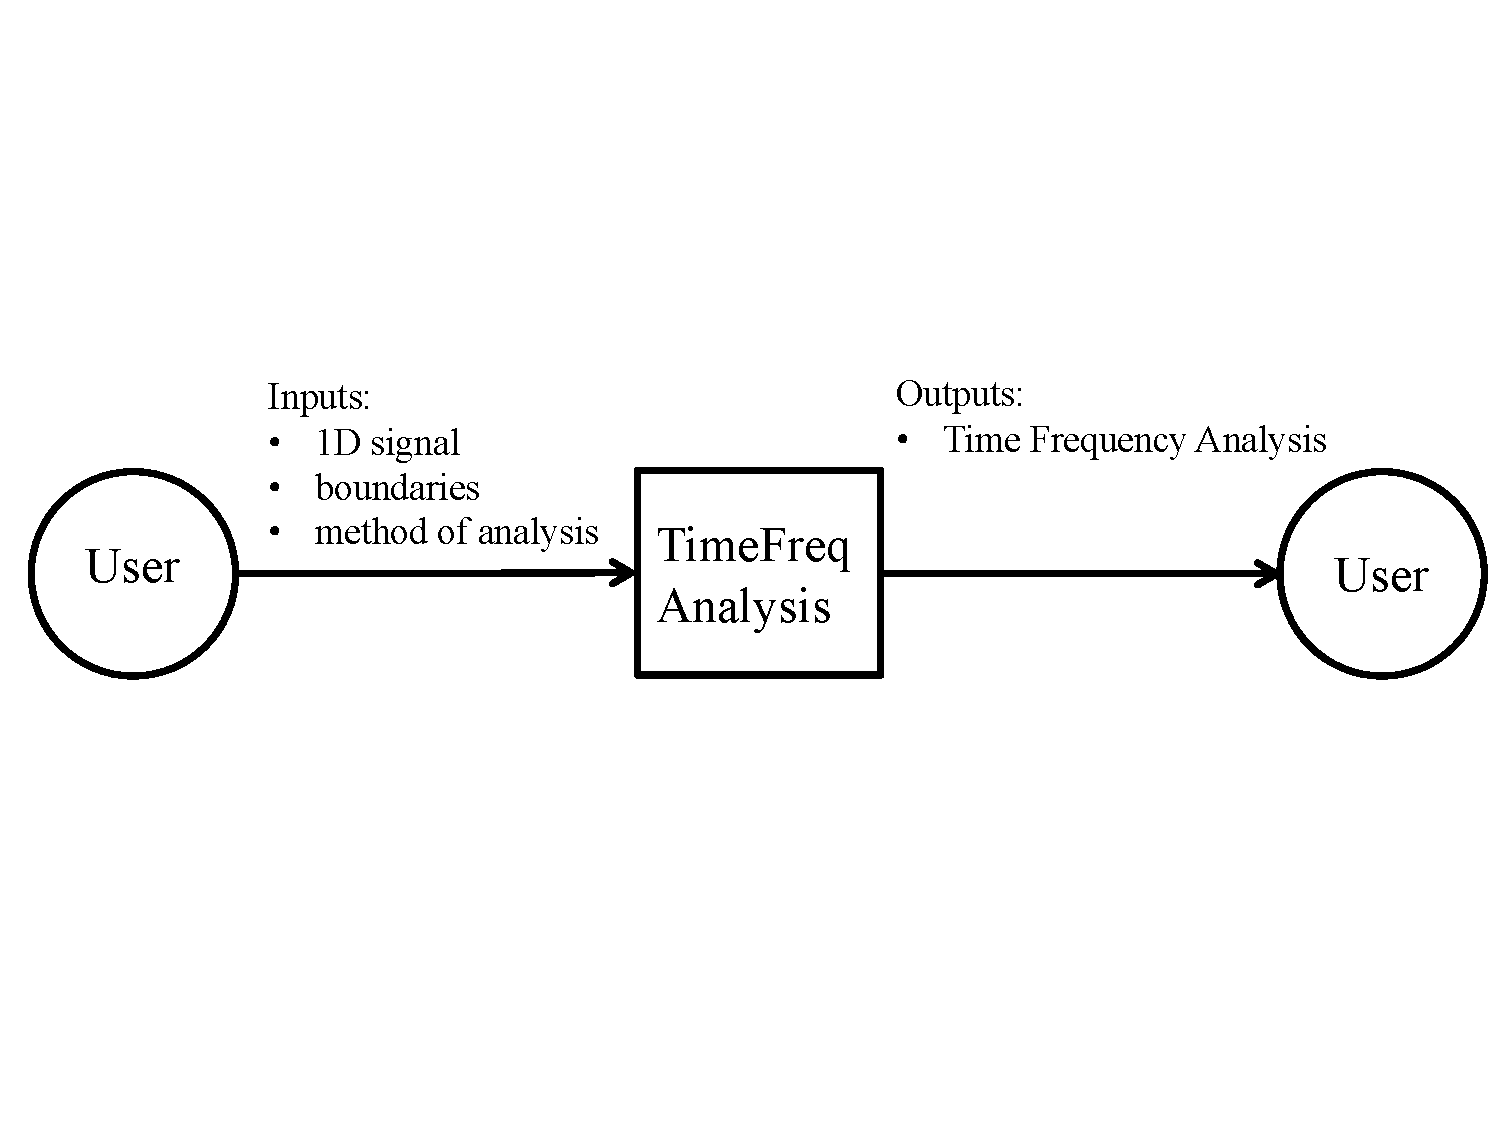
\includegraphics[width=0.6\textwidth]{SystemContextFigure}
\caption{System Context}
\label{Fig_SystemContext} 
\end{center}
\end{figure}

\begin{itemize}
\item User Responsibilities:
\begin{itemize}
\item Provide the input data, ensuring it is in correct format.
\item Enter other input variables if defaults are not appropriate.
\end{itemize}
\item \progname{} Responsibilities:
\begin{itemize}
\item Detect data type mismatch, such as a string of characters instead of a
  floating point number.
\item Detect if input data sample is too short for analysis.
\item Ensure analysis boundaries are an appropriate size for the sample.
\item Calculate the output.
\end{itemize}
\end{itemize}

\subsection{User Characteristics} \label{SecUserCharacteristics}
 
  The end user of \progname{} should have a good understanding of signal processing and Fourier transforms, ideally with a graduate level class in the area. 

\subsection{System Constraints}

There are no known constraints for this system at the present time. 

\section{Specific System Description}

This section first presents the problem description, which gives a high-level
view of the problem to be solved.  This is followed by the solution characteristics
specification, which presents the assumptions, theories, definitions and finally
the instance models. 

\subsection{Problem Description} \label{Sec_pd}

\progname{} is a computer program that is intended to transform any one dimensional signal into a two dimensional time-frequency representation of that signal, time localizing the frequencies of the signal. 

\subsubsection{Terminology and  Definitions}

This subsection provides a list of terms that are used in the subsequent
sections and their meaning, with the purpose of reducing ambiguity and making it
easier to correctly understand the requirements:

\begin{itemize}
\item Time-frequency analysis/transform - Representing and understanding a 1D signal by its time localized frequency content.
\item Short Time Fourier Transform - A method of time-frequency transform using discrete Fourier transforms.
\item Wavelet - A function that represents a portion of a `wave' or periodic function, it is mainly 0 over its domain expect for around 0, the maximum amplitude should be 1.
\item Wavelet Transform - A method of time-frequency transform using wavelets.

\end{itemize}

\subsubsection{Goal Statements} \label{goal_state}

\noindent Given a one dimensional input signal, a minimum frequency, a maximum frequency, and a time period within the recording the goal is:

\begin{itemize}

\item[GS\refstepcounter{goalnum}\thegoalnum \label{G_meaningfulLabel}:] Compute the STFT representation of the data.

\end{itemize}

\subsection{Solution Characteristics Specification}

The instance models that govern \progname{} are presented in
Subsection~\ref{sec_instance}.  The information to understand the meaning of the
instance models and their derivation is also presented, so that the instance
models can be verified.

\subsubsection{Assumptions} \label{sec_assumpt}

This section simplifies the original problem and helps in developing the
theoretical model by filling in the missing information for the physical
system. The numbers given in the square brackets refer to the theoretical model
[T], general definition [GD], data definition [DD], instance model [IM], or
likely change [LC], in which the respective assumption is used.

\begin{itemize}

\item[A\refstepcounter{assumpnum}\theassumpnum \label{mintime_assum}:] The input signal is longer than the time period over which the time-frequency analysis is computed (Ref by DD\ref{DD_stftmatrix}, IM\ref{IM1}, LC\ref{LC_user_input}).
\item[A\refstepcounter{assumpnum}\theassumpnum \label{minfreq_assum}:] The minimum frequency of the analysis is significantly larger than the sampling frequency of the input signal (Ref by DD\ref{DD_stftmatrix},DD\ref{DD_wavelet}, ,IM\ref{IM1}, LC\ref{LC_user_input}).
\item[A\refstepcounter{assumpnum}\theassumpnum \label{maxfreq_assum}:] The maximum frequency of the analysis is significantly smaller than the $1/P$ where P is the time period of the analysis (Ref by DD\ref{DD_stftmatrix}, IM\ref{IM1}, LC\ref{LC_user_input}).
\item[A\refstepcounter{assumpnum}\theassumpnum \label{representation_assum}:]The recording of the signal is an accurate representation of the signal it represents, it is not missing data points nor does it contain anomalies.(Ref by DD\ref{DD_stftmatrix}, IM\ref{IM1}).
\item[A\refstepcounter{assumpnum}\theassumpnum \label{morelet_assum}:]A morelet wavelet will be a sufficient wavelet to compute the time-frequency analysis of a signal $x(n)$. Currently, it is the only wavelet being considered for the wavelet transform, but there are other options available (Ref by IM\ref{IM1}, LC\ref{LC_onlymorelet}, LC\ref{LC_sigma}).
\item[A\refstepcounter{assumpnum}\theassumpnum \label{P_assum}:]The discrete sampling period of the signal $x(n)$ is known (Ref by DD\ref{DD_stftmatrix}, IM\ref{IM1}).

\end{itemize}

\subsubsection{Theoretical Models}\label{sec_theoretical}

This section focuses on the general equations and laws that \progname{} is based
on. 

 \noindent
\begin{minipage}{\textwidth}
\renewcommand*{\arraystretch}{1.5}
\begin{tabular}{| p{\colAwidth} | p{\colBwidth}|}
\hline
\rowcolor[gray]{0.9}
Number& T\refstepcounter{theorynum}\thetheorynum \label{T_dtft}\\
\hline
Label &\bf Discrete-time Fourier transform\\
 \hline
SI Units& N/A\\
\hline
Equation& $ X(\omega) = \displaystyle \sum_{n= 0}^{N-1} x(n) e^{-i \omega n} $ \\
\hline 
Description &
The discrete-time Fourier transform transforms a discrete signal $x(n), n[0, \ldots, N]$ into a function of frequency $X(\omega)$. \\
\hline
  Source & \url{https://cpb-us-w2.wpmucdn.com/sites.gatech.edu/dist/5/462/files/2016/08/DFT-of-Noise.pdf} \\
  \hline
  Ref.\ By & T\ref{T_stft}\\
  \hline
\end{tabular}
\end{minipage}\\

~\newline

\noindent
\begin{minipage}{\textwidth}
\renewcommand*{\arraystretch}{1.5}
\begin{tabular}{| p{\colAwidth} | p{\colBwidth}|}
  \hline
  \rowcolor[gray]{0.9}
  Number& T\refstepcounter{theorynum}\thetheorynum \label{T_stft}\\
  \hline
  Label&\bf Short Time Fourier Transform (Discrete)\\
  \hline
  Equation &  $X(n, \omega) = \displaystyle \sum_{m=-\infty}^{\infty} x(m) w(m -n) e^{-i \omega m}$\\
  \hline
  Description &  
                The above equation
                of represents the transformation from a signal $x(n)$ to a function $X(n, \omega)$ which gives the frequency content of frequency $\omega$ at discrete time $n$. $w(n)$ is the \emph{analysis window} which is normalized such that $w(0) = 1$ and $w(n \rightarrow \infty) = w(n \rightarrow - \infty) = 0$\\
  \hline
  Source & \cite{Portnoff}\\
  % The above web link should be replaced with a proper citation to a publication
  \hline
  Ref.\ By & DD\ref{DD_stftmatrix}\\
  \hline
\end{tabular}
\end{minipage}\\

~\newline

  \noindent
\begin{minipage}{\textwidth}
\renewcommand*{\arraystretch}{1.5}
\begin{tabular}{| p{\colAwidth} | p{\colBwidth}|}
\hline
\rowcolor[gray]{0.9}
Number& T\refstepcounter{theorynum}\thetheorynum \label{T_wavelet}\\
\hline
Label &\bf Wavelets and their properties\\
\hline
Equation & Let $\psi (t)$ represent the mother wavelet. \\
		& The child wavelets are $ \psi_{a,b}(t) = \frac{1}{\sqrt{a}} \psi(\frac{t-b}{a} )$
	  where $a$ is positive and defines the scale and $b$ is a real number that defines the shift.\\
\hline
Description & A wavelet is a brief oscillation constructed from any periodic function. Child wavelets are versions of the mother wavelet that have been scaled and shifted in time.
\\
\hline
  Source & \url{https://cpb-us-w2.wpmucdn.com/sites.gatech.edu/dist/5/462/files/2016/08/DFT-of-Noise.pdf}\\
  \hline
  Ref.\ By & DD\ref{DD_wavelet}\\
  \hline
\end{tabular}
\end{minipage}\\


\subsubsection{Data Definitions}\label{sec_datadef}

This section collects and defines all the data needed to build the instance
models.

\noindent
\begin{minipage}{\textwidth}
\renewcommand*{\arraystretch}{1.5}
\begin{tabular}{| p{\colAwidth} | p{\colBwidth}|}
\hline
\rowcolor[gray]{0.9}
Number& DD\refstepcounter{datadefnum}\thedatadefnum  \label{DD_morlet}\\
\hline
Label &\bf Morlet Wavelets\\
\hline
Symbol & $\psi_{Mor} (t)$\\
\hline
Equation &  $\psi_{Mor} (t) = c_\sigma \pi^{-\frac{1}{4} e^{- \frac{1}{2} t}} (e^{i \sigma t} - \kappa_\sigma)$ 

where $ \kappa_\sigma = e^{1 \frac{1}{2} \sigma^2}$  and  $c_\sigma = (1 + e^{- \sigma^2} - 2 e^{- \frac{3}{4} \sigma^2})^{\frac{1}{2}}$ \\
\hline
Description & A Morelet wavelet is one option of wavelet to be used to analyse the signal with the wavelet transform in \ref{IM_wavelet}. Here $\sigma$ is a tuning parameter that allows for a trade off between time-frequency resolutions, conventionally $\sigma < 5$.
\\
\hline
  Source &  \url{https://cpb-us-w2.wpmucdn.com/sites.gatech.edu/dist/5/462/files/2016/08/DFT-of-Noise.pdf}\\
  \hline
  Ref.\ By & DD\ref{DD_wavelet}\\
  \hline
\end{tabular}
\end{minipage}\\

\noindent
\begin{minipage}{\textwidth}
\renewcommand*{\arraystretch}{1.5}
\begin{tabular}{| p{\colAwidth} | p{\colBwidth}|}
\hline
\rowcolor[gray]{0.9}
Number& DD\refstepcounter{datadefnum}\thedatadefnum \label{DD_stftmatrix}\\
\hline
Label &\bf Matrix representation of STFT\\
\hline
Equation& for a signal $x(n)$ with a corresponding STFT $X(n, \omega)$ the matrix representation is

 $M (x(n)) = 
\begin{bmatrix}
X(n_0, \omega_0) & X( n_1 , \omega_0) & \dots & T n_N, \omega_0) \\
X( n_0, \omega_1) & X( n_1 , \omega_1) & \dots & TX(n_N, \omega_1) \\
\vdots & \vdots &\ddots & \vdots \\
X( n_0, \omega_F) & X(n_1 , \omega_F)& \dots & X( n_N, \omega_F)\\
\end{bmatrix}$
\\
\hline
Description &
For a signal $x(n)$ the matrix at $M_{a,b}(x(n)) = X(n_a, \omega_b)$. The frequency $\omega_0$ will be the minimum frequency that should be analysed and $\omega_F$ will be the maximum frequency that should be analysed, with the remaining frequencies evenly spaced intervals.
\\
\hline
  Source &  N/A\\
  \hline
  Ref.\ By & DD\ref{DD_wavelet}\\
  \hline
\end{tabular}
\end{minipage}\\

~\newline

\noindent
\begin{minipage}{\textwidth}
\renewcommand*{\arraystretch}{1.5}
\begin{tabular}{| p{\colAwidth} | p{\colBwidth}|}
  \hline
  \rowcolor[gray]{0.9}
  Number& DD\refstepcounter{datadefnum}\thedatadefnum \label{DD_wavelet}\\
  \hline
  Label&\bf Matrix representation of Wavelet Transform\\
  \hline
  Equation &  The wavelet coefficients are $ WT_\psi\{f(n)\} (a,b) = \langle f, \psi_{a,b} \rangle $. Thus, the matrix representation will be  
  
$M (x(n)) = 
\begin{bmatrix}
\langle f, \psi_{n_0,\omega_0} \rangle  & \langle f, \psi_{n_1,\omega_0} \rangle  & \dots & \langle f, \psi_{n_N,\omega_0} \rangle  
\\
\langle f, \psi_{n_0,\omega_1} \rangle  & \langle f, \psi_{n_1,\omega_1} \rangle  & \dots & \langle f, \psi_{n_N,\omega_1} \rangle  
\\
\vdots & \vdots &\ddots & \vdots \\
\langle f, \psi_{n_0,\omega_F} \rangle  & \langle f, \psi_{n_1,\omega_F} \rangle  & \dots & \langle f, \psi_{n_N,\omega_F} \rangle  
\end{bmatrix}$
\\ \\
  \hline
  Description & The wavelet coefficients can be assembled into a matrix for a time-frequency representation of the signal. The frequency $\omega_0$ will be the minimum frequency that should be analysed and $\omega_F$ will be the maximum frequency that should be analysed, with the remaining frequencies evenly spaced intervals. \\
  \hline
  Source & \url{https://en.wikipedia.org/wiki/Wavelet}\\
  % The above web link should be replaced with a proper citation to a publication
  \hline
  Ref.\ By & DD\ref{IM1}\\
  \hline
\end{tabular}
\end{minipage}\\

\subsubsection{Instance Models} \label{sec_instance}    

This section transforms the problem defined in Section~\ref{Sec_pd} into 
one which is expressed in mathematical terms. It uses concrete symbols defined 
in Section~\ref{sec_datadef} to replace the abstract symbols in the models 
identified in Section~\ref{sec_theoretical}.

The goal statement \ref{goal_state} is solved by IM\ref{IM1}. 
~\newline

%Instance Model 1
~\newline
\noindent
\begin{minipage}{\textwidth}
\renewcommand*{\arraystretch}{1.5}
\begin{tabular}{| p{\colAwidth} | p{\colBwidth}|}
  \hline
  \rowcolor[gray]{0.9}
  Number& IM\refstepcounter{instnum}\theinstnum \label{IM1}\\
  \hline
  Label& \bf Time-frequency representation of a signal $x(n)$\\
  \hline
  Input& $x(n)$, $T$,  $n_i$, $\Delta_n$, $\omega_{min}$, $\omega_{max}$ and a method to compute the time frequency representation $T$ where $T \in{S,W}$, $S$ for a STFT and $W$ for a wavelet transform.\\
  \hline
  Output& $M(x(n))$ from $n[ni, \ldots, ni + \Delta_n]$ and from $\omega[\omega_{min} , \ldots , \omega_{max}]$\\ 
  \hline
  Description&$x(n)$: discrete input signal of length N, $n[0, \ldots, N]$ \\
  &$P$: sampling period of $x(n)$ (\si{\second})\\
  &$n_i$: discrete time within signal to begin time-frequency transform\\
  &$\Delta_n$: the length of the time period over which the transform is performed. \\
  &$\omega_{min}$: the minimum frequency analysed for the transform (Hz).\\
  &$\omega_{max}$: the maximum frequency analysed for the transform (Hz).\\
  &$M ((x(n))$: the matrix representing of the time-frequency transform of $x(n)$.
  \\
  \hline
  Sources & N/A \\
  \hline
  Ref.\ By &  R\ref{R_inputs}, R\ref{R_illegal_input}, R\ref{R_OutputInputs}\\
  \hline
\end{tabular}
\end{minipage}\\

%~\newline


\subsubsection{Input Data Constraints} \label{sec_DataConstraints}    

Table~\ref{TblInputVar} shows the data constraints on the input output
variables.  The column for physical constraints gives the physical limitations
on the range of values that can be taken by the variable.  The column for
software constraints restricts the range of inputs to reasonable values.  The
software constraints will be helpful in the design stage for picking suitable
algorithms.  The constraints are conservative, to give the user of the model the
flexibility to experiment with unusual situations.  The column of typical values
is intended to provide a feel for a common scenario.  The uncertainty column
provides an estimate of the confidence with which the physical quantities can be
measured.  This information would be part of the input if one were performing an
uncertainty quantification exercise.

\begin{table}[!h]
  \caption{Input Variables} \label{TblInputVar}
  \renewcommand{\arraystretch}{1.2}
\noindent \begin{longtable*}{l l l l c} 
  \toprule
  \textbf{Var} & \textbf{Physical Constraints} & \textbf{Software Constraints} &
                             \textbf{Typical Value} & \textbf{Uncertainty}\\
  \midrule 
  $n_i$ & $ 0 \leq n_i \leq (N - \Delta_n) $ & N/A & 26 & N/A*
  \\
  $\Delta_n$ & $ 0 < \Delta_n$ , $ t_i + \Delta_n \leq N$ & N/A & 2000 & N/A \text{*} 
  \\
  $\omega_{min}$ & $ 0 < \omega_{min} << \omega_{max}$ & $  1/\Delta_n << \omega_{min} << 1/P $ & 2 Hz & N/A \text{*} \\
    $\omega_{max}$ & $ \omega_{min} << \omega_{max} $ & $  1/\Delta_n << \omega_{max} << 1/P $ & 200 Hz & N/A \text{*} \\
   $ x(n) $ & N/A & $ x_{min} \leq x(n) \leq x_{max}$ for all n & 0.03627 & 10\%\\
   $P$ & $P > 0$ & N/A & 0.25 \si{\second} & 10\% \\
\bottomrule \\
\end{longtable*}
\end{table}

\noindent 
\begin{description}
\item[(*)] The input discrete time indexes and frequencies do not have an uncertainty in the context of this project. They are merely the boundaries for the time-frequency transformed to be performed within, it would not effect the accuracy of the transform, just the portion of the signal it is performed upon.
\item[(**)] $P$ is determined by the method of recording/sampling. It is not chosen by the user but the user must specify it.
\end{description}

\subsubsection{Properties of a Correct Solution} \label{sec_CorrectSolution}

\noindent
The output of this \progname{} is a time-frequency \emph{representation} of a 1D signal. What is important to recognize is that a `representation' really could be anything, and therefore what could be considered a `correct solution' is quite diverse and subjective. A correct solution should look like a heat map when graphed, essentially the matrix values should not be 'random' or sporadically scattered, and there should be 'clusters' at the prominent frequencies at the time they occur.The output should obviously be consistent for the same input signal and similar for similar input signals, which seems trivial but will be useful when testing to determine what a correct output can be defined as. Expressed in table \ref{TblOutputVar} any one value in a transform cannot be greater than the value of the signal itself, at the same time $n$, since that would violate the principals of transforms outlined by T\ref{T_dtft}, T\ref{T_stft}, and T\ref{T_wavelet}.

\begin{table}[!h]
\caption{Output Variables} \label{TblOutputVar}
\renewcommand{\arraystretch}{1.2}
\noindent \begin{longtable*}{l l} 
  \toprule
  \textbf{Var} & \textbf{Physical Constraints} \\
  \midrule 
  $M_{a,b}$ & $ M_{n,b}\ \leq x(n) $
  \\
  \bottomrule
\end{longtable*}
\end{table}

\section{Requirements}

This section provides the functional requirements, the business tasks that the
software is expected to complete, and the nonfunctional requirements, the
qualities that the software is expected to exhibit.

\subsection{Functional Requirements}

\begin{itemize}

\item[R\refstepcounter{reqnum}\thereqnum \label{R_Inputs}:] Program shall take the signal to be analyzed as input. All other inputs (as specified in table \ref{TblInputVar}) will have defaults, but program shall accept user inputs for those as well (IM \ref{IM1}).

\item[R\refstepcounter{reqnum}\thereqnum \label{R_illegal_input}:] Program shall notify user if an input value is illegal or out of bounds (IM \ref{IM1}).
  
\item[R\refstepcounter{reqnum}\thereqnum \label{R_OutputInputs}:] The output shall be a time frequency representation of the signal in the specified time period and over the specified frequency range (IM \ref{IM1}).

\item[R\refstepcounter{reqnum}\thereqnum \label{R_spectral_leakage}:] The program should minimize spectral leakage (IM \ref{IM1}, DD\ref{DD_wavelet}, DD\ref{DD_morlet}). 

\item[R\refstepcounter{reqnum}\thereqnum \label{R_VerifyOutput}:] The time-frequency representations of simple input signals (such as sinusoids of a constant frequency or an impulse) should be comparable to existing time-frequency transforms of that signal (IM \ref{IM1}).

\end{itemize}

\subsection{Nonfunctional Requirements}

\begin{itemize}
\item[R\refstepcounter{reqnum}\thereqnum \label{R_heatmap}:] Program shall plot time-frequency representation as a heat map.
\item[R\refstepcounter{reqnum}\thereqnum \label{R_timecomplexity}:] The time complexity for this program should be $O(n)$,
\item[R\refstepcounter{reqnum}\thereqnum \label{R_useability}:] Program will not have a graphical user interface but should still be easy to use, the input parameters besides the signal shall all have default values, there should be at most 6 optional inputs.
\item[R\refstepcounter{reqnum}\thereqnum \label{R_readability}:] The program code should be clear and readable.
\item[R\refstepcounter{reqnum}\thereqnum \label{R_integration}:] The program should easily integrate with other software programs. 
\end{itemize}

\section{Likely Changes}    

\noindent \begin{itemize}
    
\item[LC\refstepcounter{lcnum}\thelcnum\label{LC_onlymorelet}:]  Currently there is only one option for type of wavelet: a Morlet wavelet. Depending on the resources available, the type of wavelet could be specified, as many different wavelets exist that all do slightly different things. This will have to be added as an input IF the user chooses wavelet transform for the input $T$ as in table \ref{TblInputVar}. Essentially, this would be a conditional input, only if the user selects wavelet transform. Per assumption A\ref{morelet_assum}.

\item[LC\refstepcounter{lcnum}\thelcnum\label{LC_sigma}:]  $\sigma$ a parameter used by the Morlet wavelet transform \ref{DD_morlet} can not be set by the user, as the end goal of this program is to analyse a large among of similar signals and then compare them, and $\sigma$ should remain constant for all of those signals. However, it may be beneficial for the user to be able to input this parameter to find the best time-frequency resolution for their problem.

\item[LC\refstepcounter{lcnum}\thelcnum\label{LC_user_input}:] Currently, the user specifies the following four input parameters: $n_i$, $\Delta_n$, $\omega_{min}$ and $\omega_{max}$. However, this could lead to the user inputting inappropriate values for the sample. A time-frequency at too small an interval will not yield useful results, but this depends on the content of the sample itself, so it cannot be a parameter set by the system. However, it might be fit to restrict the range of these input values more then they already are. 

\end{itemize}


\section{Traceability Matrices and Graphs}

The purpose of the traceability matrices is to provide easy references on what
has to be additionally modified if a certain component is changed.  Every time a
component is changed, the items in the column of that component that are marked
with an ``X'' may have to be modified as well.  Table~\ref{Table:trace} shows the
dependencies of theoretical models, general definitions, data definitions, and
instance models with each other. Table~\ref{Table:R_trace} shows the
dependencies of instance models, requirements, and data constraints on each
other. Table~\ref{Table:A_trace} shows the dependencies of theoretical models,
general definitions, data definitions, instance models, and likely changes on
the assumptions.

\afterpage{
\begin{landscape}
\begin{table}[h!]
\centering
\begin{tabular}{|c|c|c|c|c|c|c|}
\hline
	& \aref{mintime_assum}& \aref{minfreq_assum}& \aref{maxfreq_assum}& \aref{representation_assumm}& \aref{morelet_assum}& \aref{P_assum} \\
\hline
\tref{T_dtft}          & & & & & &  \\ \hline
\tref{T_wavelet}       & &X&X& & &  \\ \hline
\tref{T_stft}          & &X&X&X& &X \\ \hline
\ddref{DD_morlet}       & & & & & &  \\ \hline
\ddref{DD_stftmatrix}   &X& & & & &  \\ \hline
\iref{DD_wavelet}       & & & & & &  \\ \hline
\iref{IM1}             &X&X&X&X&X&X  \\ \hline
\lcref{LC_onlymorelet} & & & & &X&  \\ \hline
\lcref{LC_sigma}       & & & & & &  \\ \hline
\lcref{LC_user_input}  &X&X&X& & &  \\ 
\hline
\end{tabular}
\caption{Traceability Matrix Showing the Connections Between Assumptions and Other Items}
\label{Table:A_trace}
\end{table}
\end{landscape}
}

\begin{table}[h!]
\centering
\begin{tabular}{|c|c|c|c|c|c|c|c|}
\hline        
	& \tref{T_dtft} & \tref{T_wavelet}& \tref{T_stft}& \ddref{DD_morlet} & \ddref{DD_stftmatrix}& \ddref{DD_wavlet} & \iref{IM1} \\
\hline
\hline
\tref{T_dtft}          & & &X& &X& & \\ \hline
\tref{T_wavelet}       & & & & & &X& \\ \hline
\tref{T_stft}        &X& & & &X& & \\ \hline
\ddref{DD_morlet}      & & & & &X& & \\ \hline
\ddref{DD_stftmatrix}  &X& &X& & & &X\\ \hline
\ddref{DD_wavelet}     & &X& & & & &X\\ \hline
\iref{IM1}             & & & &X&X&X \\
\hline
\end{tabular}
\caption{Traceability Matrix Showing the Connections Between Items of Different Sections}
\label{Table:trace}
\end{table}
\begin{table}[h!]
\centering
\begin{tabular}{|c|c|}
\hline
	& \iref{IM1} \\
\hline
\rref{R_Inputs}        &X \\ \hline
\rref{R_illegal_input} &X \\ \hline
\rref{R_OutputInputs}  &X  \\ \hline
\rref{R_spectral_leakage}&X \\ \hline 
\rref{R_VerifyOutput}  &X \\ 
\hline
\end{tabular}
\caption{Traceability Matrix Showing the Connections Between Requirements and Instance Models}
\label{Table:R_trace}
\end{table}

% \begin{figure}[h!]
% 	\begin{center}
% 		%\rotatebox{-90}
% 		{
% 			\includegraphics[width=\textwidth]{ATrace.png}
% 		}
% 		\caption{\label{Fig_ATrace} Traceability Matrix Showing the Connections Between Items of Different Sections}
% 	\end{center}
% \end{figure}


% \begin{figure}[h!]
% 	\begin{center}
% 		%\rotatebox{-90}
% 		{
% 			\includegraphics[width=0.7\textwidth]{RTrace.png}
% 		}
% 		\caption{\label{Fig_RTrace} Traceability Matrix Showing the Connections Between Requirements, Instance Models, and Data Constraints}
% 	\end{center}
% \end{figure}

~\newpage

\bibliographystyle {plainnat}
\bibliography {../../refs/References}

\end{document}